%!TEX root = main.tex

\section*{Introduction}

Genetic markers have long been used in the 
management of Pacific salmon, and salmon conservation and management has been
a driving force behind a number of advances in molecular ecology,
from data generation techniques \citep{clemento2011discovery,campbell2015genotyping,mckinney2017managing}
to statistical methodology
\citep{smouse1990genetic,anderson2002model,pella2006gibbs}.
Two broadly applicable innovations that have been
actively fostered by the Pacific salmon research community are genetic
stock identification
(GSI:~\citealt{milner1982genetic,beacham2004dna,seeb2007development})
and parentage based tagging
(PBT:~\citealt{anderson2006power, garza2007large, abadia2013large, steele2013validation}).  



 In the 1980's, electrophoretically
detectable genetic variation, in the form of allozymes
\citep{ayala1972allozymes,allendorf1981use}, was used to
establish a program of GSI for Chinook salmon,
{\em Oncorhynchus tshawytscha} \citep{milner1982genetic}.  Extensive sampling
revealed that these allozyme markers
exhibited different allele frequencies among major stocks of Chinook salmon on the West Coast.
These allele frequency differences make GSI possible, and
\citet{milner1985genetic} soon showed that proportions of stocks in
the Washington state coastal troll fishery could be estimated by GSI.
Since that time, with the development of novel molecular markers, and, now
with increasing capacity to sequence genomic material, the scope and scale of GSI
has expanded considerably.

By using greater numbers of more variable markers than the allozymes available
in the 1980s it is possible to accurately
identify the population of origin of individual fish, rather than simply estimating
aggregated stock proportions.  It is also possible to resolve populations of fish that
are much more closely related than before.  Furthermore, reference data sets with genotypes
from hundreds of populations throughout the range of multiple species of salmon and
other anadromous species
\citep{seeb2007development,gilbey2018microsatellite,barclay2019genetic} now exist, and are routinely used to assign fish caught thousands of
kilometers from their natal streams to their stock of origin. Applications include estimating fishery
composition \citep{satterthwaite2015stock}, providing real-time information for genetics-informed fishery closures \citep{beacham2004dna}, assessing the spatial distribution of different stocks in the
ocean \citep{urawa2009stock} and their temporal distribution in upstream migrations
\citep{hess2014monitoring},  and monitoring  bycatch \citep{hasselman2016genetic} or illegal captures \citep{wilmot1999origins} in marine fisheries.

Although sequencing costs continue to decline, they are high enough
that there remains a tradeoff
between reference baselines that include information from a large number of
populations across a broad scale, and those that have been tailored
to distinguish between closely related populations on a smaller, regional scale.
Because of cost considerations, reference baselines that include populations across a broad 
spatial scale may include only a few populations from each sub-region.  Furthermore,
baselines tailored to a specific region often assemble markers that specifically
show allele frequency differences between the closely related---and hence difficult
to resolve---stocks within the region.  Consequently, regionally targeted baselines typically
outperform broad-scale baselines in resolving populations within the region.

The ascendance over the last decade of parentage based tagging (PBT) as a management
tool for Pacific salmon adds another factor to consider when developing a GSI baseline.
Since the first proposal \citep{anderson2005description} to replace or augment the coded-wire tag
programme \citep{nandor2010overview}
with PBT, it has been noted that one of the major advantages of a genetic program for
PBT is that the genetic markers used for PBT could also be useful for GSI (and
vice versa).  This 

Here, we present a reference baseline for Chinook salmon, targeted to the complex population 
structure within the Central Valley of California. Chinook salmon of the two main river basins---the 
Sacramento and the San Joaquin---within the Central Valley exhibit the greatest run-timing diversity
within the species.  With four recognized ecotypes, delineated primarily on the basis of run timing
(fall-, late-fall-, winter-, and spring-run), adult Chinook salmon can be found migrating or residing
in freshwater every month of the year in California. NEED MORE HERE. Certainly we should cite
\citet{yoshiyama1998historical}.


 \section*{Methods}

More verbiage

\subsection*{Population Sampling}

We sampled fish for the reference baselines from XX locations across California.
These locations included sites in the two
main tributaries (the Sacramento River and the San Joaquin River) within
California's Central Valley, the Klamath-Trinity basin in Northern California, and
3 rivers of the California coast (Russian, Eel, etc)
(Fig.~\ref{fig:map}).
%%%%%%%%%%%%%
\begin{figure}
\newcommand{\mapcap}{\footnotesize  A map of sampling locations represented in the reference 
baseline.  The colored circles aside
each location name represent the different run-timing groups of Chinook salmon
included in the collections from the location.  Color codes are as follows: \Wball~=~Winter run,
\LFball{}~=~Late-fall run, \Fball~=~Fall run, \Sball~=~Spring run. Abbreviations used in location names as folows: R. = River; Ck. = Creek; H. = Hatchery; NFH = National Fish Hatchery.}
\begin{center}
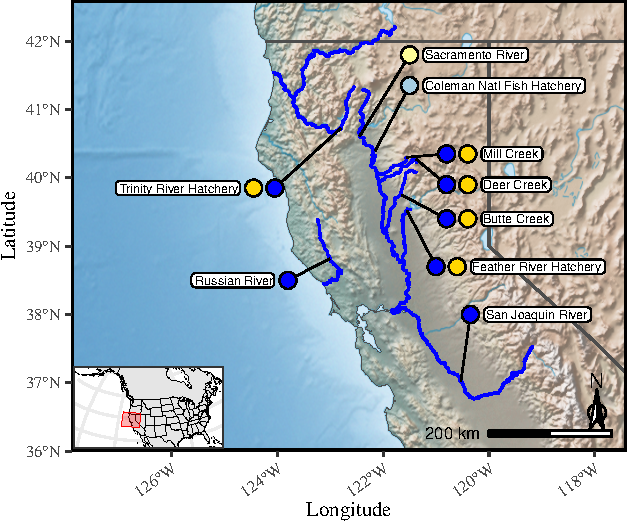
\includegraphics[width=\columnwidth]{images/map-crop.pdf}
\end{center}
\caption[\mapcap]{\mapcap}
\label{fig:map}
\end{figure}
%%%%%%%%%%%%%%%
Collections in each location were separated into fish from the different run-timing ecotypes according
to a variety of criteria. The last vestiges of winter-run Chinook salmon are maintained at the Livingston
Stone National Fish Hatchery for supplementation (released as juveniles into the river) and as a captive broodstock;
sampling was performed by hatchery staff during spawning.   
(We need to talk about how these were split into spring run, fall-run, winter 
run, etc.
In total, the samples in the baseline represent fish from five different Evolutionarily Significant 
Units (ESUs) of Chinook salmon \citep{waples1991pacific} A summary of the different collections 
%%%%%%%%%%%%%%%%
\begin{table*}
\caption{\footnotesize Collections of fish in the reference baseline.  The Sampling Months column shows
a pictorial representation of the proportion of each collection sampled in each month.  Colors in
this column correspond to run-timing groups as described in the caption of Fig.~\protect\ref{fig:map}.}
{\small 
\begin{tabular*}{\linewidth}{@{\extracolsep{\fill}} lllllrcr}
\hline\hline\vspace*{0.4ex}
Mainstem River$^1$&Code&Location Name$^2$&Run&Reporting Unit$^4$&ESU$^4$&$N$&$N_\mathrm{day}^5$&Sampling Months&Year Range\tabularnewline
\hline Rogue R.&CRHS&Cole Rivers H.&Spring&SO-NCal-Coast&SONCC&50&0&\raisebox{-0.12 em}{
\includegraphics[height=1.02em]{../tex/images/months-CRHS_Cole-Rivers-Hatchery.pdf}}&2004--2010\tabularnewline
Smith R.&SmRF&Smith R.&Fall&SO-NCal-Coast&SONCC&46&46&\raisebox{-0.12 em}{
\includegraphics[height=1.02em]{../tex/images/months-SmRF_Smith-River.pdf}}&2010--2011\tabularnewline
Klamath R.&BCkF&Blue Ck.&Fall&SO-NCal-Coast&SONCC&56&56&\raisebox{-0.12 em}{
\includegraphics[height=1.02em]{../tex/images/months-BCkF_Blue-Creek.pdf}}&2008--2008\tabularnewline
Klamath R.&IGHF&Iron Gate H.&Fall&Klamath-Trinity&UKTR&93&92&\raisebox{-0.12 em}{
\includegraphics[height=1.02em]{../tex/images/months-IGHF_Iron-Gate-Hatchery.pdf}}&2017--2017\tabularnewline
Trinity R.&TRS&Trinity R. H.&Spring&Klamath-Trinity&UKTR&46&46&\raisebox{-0.12 em}{
\includegraphics[height=1.02em]{../tex/images/months-TRS_Trinity-River-Hatchery.pdf}}&2012--2012\tabularnewline
Trinity R.&TRF&Trinity R. H.&Fall&Klamath-Trinity&UKTR&41&41&\raisebox{-0.12 em}{
\includegraphics[height=1.02em]{../tex/images/months-TRF_Trinity-River-Hatchery.pdf}}&2012--2012\tabularnewline
Eel R.&ERF&Eel R.&Fall&Cent-Cal-Coast&CCC&93&0&\raisebox{-0.12 em}{
\includegraphics[height=1.02em]{../tex/images/months-ERF_Van-Arsdale-Fisheries-Station.pdf}}&2014--2014\tabularnewline
Russian R.&RRF&Warm Springs H.&Fall&Cent-Cal-Coast&CCC&92&92&\raisebox{-0.12 em}{
\includegraphics[height=1.02em]{../tex/images/months-RRF_Warm-Springs-Hatchery.pdf}}&2012--2012\tabularnewline
Sacramento R.&SRW&Livingston Stone NFH&Winter&CV-Winter&CVWR&111&20&\raisebox{-0.12 em}{
\includegraphics[height=1.02em]{../tex/images/months-SRW_Livingston-Stone-National-Fish-Hatchery.pdf}}&2013--2014\tabularnewline
Sacramento R.&BCS&Butte Ck.&Spring&CV-Spring&CVSR&116&116&\raisebox{-0.12 em}{
\includegraphics[height=1.02em]{../tex/images/months-BCS_Butte-Creek.pdf}}&2004--2017\tabularnewline
Sacramento R.&MDS&Deer Ck.&Spring&CV-Spring&CVSR&34&34&\raisebox{-0.12 em}{
\includegraphics[height=1.02em]{../tex/images/months-MDS_Deer-Creek.pdf}}&2002--2002\tabularnewline
Sacramento R.&MDS&Mill Ck.&Spring&CV-Spring&CVSR&50&50&\raisebox{-0.12 em}{
\includegraphics[height=1.02em]{../tex/images/months-MDS_Mill-Creek.pdf}}&2002--2004\tabularnewline
Sacramento R.&FRHS&Feather R. H.&Spring&CV-Fall&CVSR&202&202&\raisebox{-0.12 em}{
\includegraphics[height=1.02em]{../tex/images/months-FRHS_Feather-River-Hatchery.pdf}}&2010--2019\tabularnewline
Sacramento R.&FRHF&Feather R. H.&Fall&CV-Fall&CVFR&106&106&\raisebox{-0.12 em}{
\includegraphics[height=1.02em]{../tex/images/months-FRHF_Feather-River-Hatchery.pdf}}&2008--2010\tabularnewline
Sacramento R.&BCF&Butte Ck.&Fall&CV-Fall&CVFR&45&45&\raisebox{-0.12 em}{
\includegraphics[height=1.02em]{../tex/images/months-BCF_Butte-Creek.pdf}}&2004--2016\tabularnewline
Sacramento R.&MDF&Deer Ck.&Fall&CV-Fall&CVFR&24&24&\raisebox{-0.12 em}{
\includegraphics[height=1.02em]{../tex/images/months-MDF_Deer-Creek.pdf}}&2002--2004\tabularnewline
Sacramento R.&MDF&Mill Ck.&Fall&CV-Fall&CVFR&49&49&\raisebox{-0.12 em}{
\includegraphics[height=1.02em]{../tex/images/months-MDF_Mill-Creek.pdf}}&2002--2004\tabularnewline
San Joaquin R.&SJRF&San Joaquin R.&Fall&CV-Fall&CVFR&79&79&\raisebox{-0.12 em}{
\includegraphics[height=1.02em]{../tex/images/months-SJRF_San-Joaquin-River.pdf}}&2016--2016\tabularnewline
Sacramento R.&CHLF&Coleman NFH&Late-fall&CV-Late-Fall&CVFR&261&261&\raisebox{-0.12 em}{
\includegraphics[height=1.02em]{../tex/images/months-CHLF_Coleman-National-Fish-Hatchery.pdf}}&2011--2015\tabularnewline

\end{tabular*}
}
\rule{3cm}{0.3pt}

{\footnotesize
$^1$R. = River.\\
$^2$Ck. = Creek; NFH = National Fish Hatchery; R. = River; H. = Hatchery.\\
$^3$ESU = Evolutionarily Significant Unit; CVFR = Central Valley Fall Run ESU; CVSR = Central Valley Spring Run ESU; CVWR = 
Central Valley Winter Run ESU; CC = California Coastal ESU; UKTR = Upper Klamath and Trinity Rivers ESU.
}
\hrule\vspace*{0.3ex}\hrule
\end{table*}
%%%%%%%%%%%%%%%%%%%%%

\subsection*{Genetic Markers}

To assemble the markers for this reference baseline, we drew upon several different
sources, as detailed in the separate sections below.

\subsubsection*{Conversion of existing SNPtype assays}

A number of SNP markers from earlier discovery efforts \citep{clemento2011discovery} had already 
been validated as useful for GSI
and PBT in California \citep{clemento2014evaluation}. These markers were originally assayed
using TaqMan (Life Technologies Corp., Carlsbad, CA) probes or SNPtype assays (CITE).
In order to type these markers using amplicon sequencing, we followed the methods in
\citet{campbell2015genotyping} and added the Illumina small RNA sequencing primer and 
read 2 sequencing primer to the SNPtype Specific Target Amplification Primer and Locus 
Specific Primers respectively.  We then dropped any loci that produced genotypes that were 
frequently inconsistent with genotypes produced with the SNPtype assays and any loci that 
did not amplify well or took over PCRs when run with the other loci in the panel.  We then 
used Freebayes \citep{garrison2012haplotype} to identify non mulltinucleotide or complex variants
in addition the the SNPs targeted by the original TaqMan assays.

\subsubsection*{Additional microhaplotype discovery}

We undertook a new discovery process to develop additional multiallelic
microhaplotype \citep{baetscher2018microhaplotypes} markers in California Chinook.
NEED TO DESCRIBE.

After we designed these loci, we compiled the reference sequences for these and the
other loci and mapped them to the Chinook v1.0 genome assembly \citep{christensen2018chinook}
with both the Burrows-Wheeler Aligner (CITE) and the BLAST-like Alignment tool \citep{kent2002blat}.
Genome locations found with both aligners were assumed to be the most likely locations
of these target amplicons in the genome.

\subsubsection*{Markers around the RoSA region of \citet{thompson2020complex}}

We include amplicons targeting SNPs within the ``Region of Strongest Assocation'' (RoSA)
between spring-run and fall-run fish described in \citet{thompson2020complex}.

Need more here.

\subsubsection*{Identifying and Designing markers from the Late-Fall Associated Region}

To identify loci with large allele frequency differences between late-fall and fall-run Chinook salmon, 
we first conducted a simple case-control GWAS using the low-coverage whole genome sequencing 
data of \citet{thompson2020complex}.  We conducted two separate association-study comparisons.  
The first involved the 16 late-fall run fish as cases with 16 fall-run fish from the Feather River Hatchery as controls. 
The second involved the same 16 late-fall fish as cases, but used 16 fall-run fish from the San 
Joaquin River as controls.  The association studies were performed for each chromosome with 
ANGSD \citep{pmid21663684,korneliussen_angsd_2014}, using the following command: {\footnotesize\tt angsd -yBin \{ybin\}  -r \{chrom\} 
-minMapQ 30 -minQ 20 -minInd 12 -doAsso 1 -GL 1 -doMajorMinor 1 -doMaf 1 -SNP\_pval 1e-6  
-out \{prefix\}  -bam \{bamlist\}}, where {\tt \{ybin\} } is the path to a file indicating the cases and 
controls, 
{\tt \{chrom\} } indicates the chromosome name, {\tt \{prefix\} } is the prefix to use for output files, and 
{\tt \{bamlist\} } is the path to the text file holding paths to the BAM files, one for each individual, ordered as in {\tt \{ybin\} }.

There was only one peak in association scores that was shared between both comparisons (see 
Results). From this peak we identified candidates for followup genotyping by including the 10 
SNPs with the lowest association p-values, and supplementing those with additional SNPs that 
showed:
\begin{itemize}
\item An estimated absolute allele frequency difference (between late-fall and all 32 fall-run fish)  $>0.75$,  with an approximate lower confidence interval of that figure of 0.5,  or
\item An estimated absolute frequency difference of >0.5 with a lower confidence interval >0.25 and 
with either fall-run or late-fall run being nearly fixed for one of the alleles, or
\item An annotation from snpEff \citep{cingolani2012program} of “HIGH” or “MODERATE”, or
\item An absolute frequency difference $>0.48$ and a lower confidence interval of $>0.25$ and a 
genomic  coordinate $> 2.2$~Mb.
\end{itemize}
The final condition was implemented to gather several SNPs within the flanking region to the right of 
the main peak of association. 

For the candidate markers found by the above process, we designed amplification primers using 
Primer3 \citep{koressaar2007enhancements,untergasser2012primer3} and tested amplification in a 
subset of Chinook salmon 
samples. The primer pairs that amplified sequence that reliably mapped back to the association-peak region were then typed
in a separate collection of 1,638 Sacramento River Chinook salmon sampled from the fish trap below Keswick Dam, including 1,169 winter run, 281 spring 
run, and 188 fall/late-fall run. We divided the fish identified as fall/late-fall via the 125-locus genetic 
stock identification data set into fall run and late fall run according to their sampling date at Keswick: 
99 fish arriving before Dec 26 were classified as fall run and 89 fish arriving after Dec 26 were 
classified as late-fall run.   The allele frequencies of the target SNPs at the remaining amplicons 
were 
estimated for each of these four groups: winter, spring, fall, and late-fall, and we retained
amplicons showing large allele frequency  differences between late-fall fish and all other runs.



\section*{Results}

\subsection*{Genetic Markers}

\subsubsection*{Late-fall Associated Region Markers}

The case-control association test revealed a single peak on chromosome 34 with large allele frequency differences
between Central Valley late-fall and fall-run fish.  This peak was evident both in the comparison of
late-fall fish to fall-run fish in the Feather River Hatchery and of late-fall fish to the fall-run fish in
the San Joaquin River (Fig.~\ref{fig:lfar-assoc}).
%%%%%%%%%%%%%%%%%%%%%
\begin{figure*}
\newcommand{\lfarcap}{\footnotesize Negative log base 10 of association $p$-values for
individual SNPs for late-fall versus fall run.  $x$ axis shows position in genome (in megabases),
with color alternating by chromosome, as indicated by numbers above the $x$-axis. ``Unk'' refers
to unplaced scaffolds in the Otsh\_v1.0 genome assembly \citep{christensen2018chinook}. The 
upper panel is the comparison between late-fall and Feather River Hatchery fall, while the lower 
panel is the comparison of late-fall to San Joaquin River fall. }
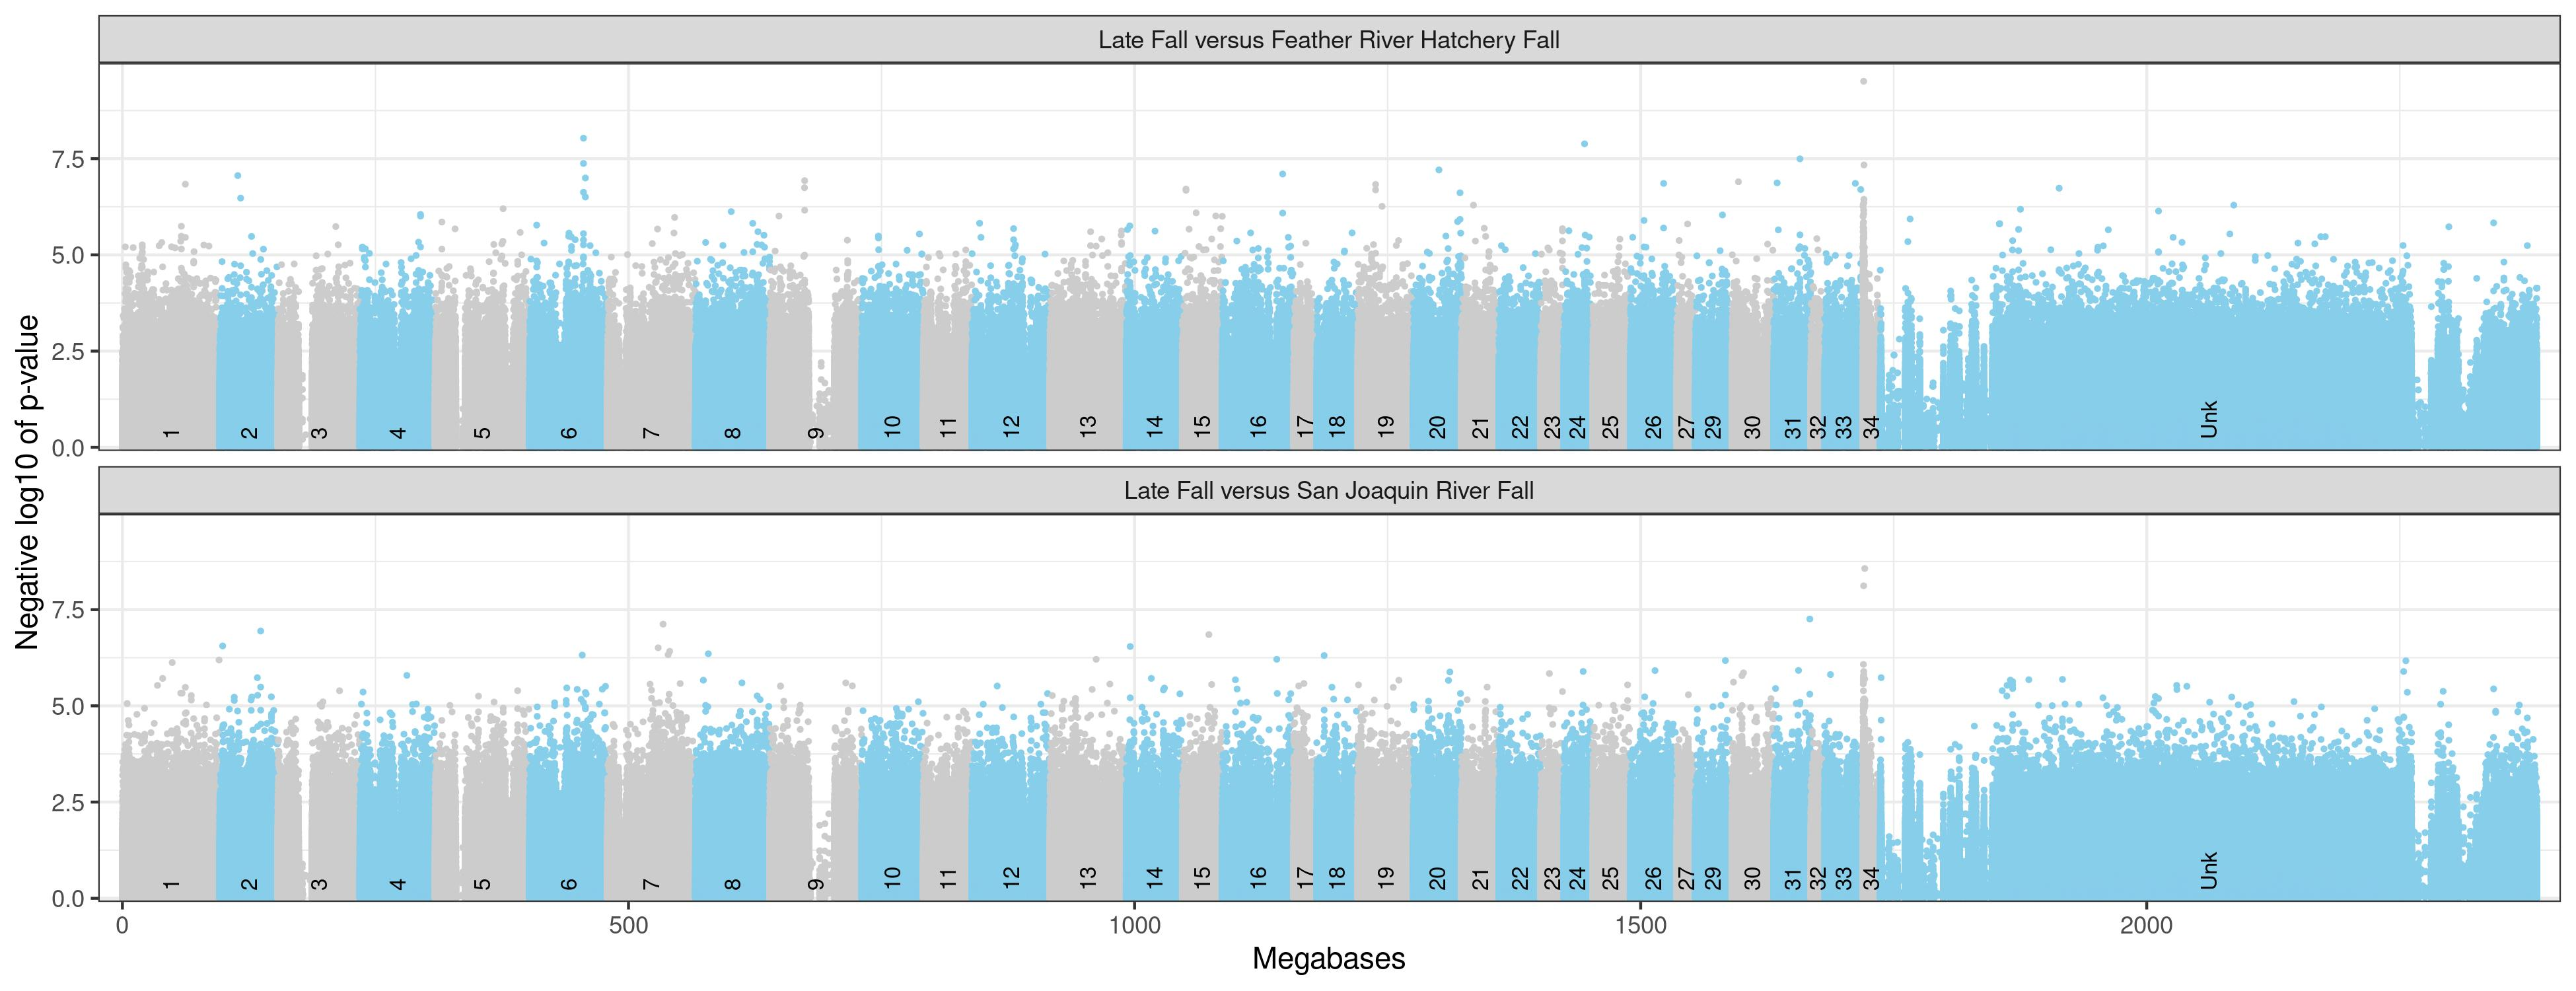
\includegraphics[width=\textwidth]{images/lfar-assoc-faceted.jpg}
\caption[\lfarcap]{\lfarcap}
\label{fig:lfar-assoc}
\end{figure*}
%%%%%%%%%%%%%%%%%%%%
The Manhattan plot of Fig.~\ref{fig:lfar-assoc} shows sporadic SNPs with low association
$p$-values.  These are not shared between the two different late-fall to fall comparisons, and
sites that we investigated were concentrated in areas of poor mapping suggesting that their
$p$-values were artifactual.  By contrast, a large number of sites near the prominent peak on
chromosome 34 had large allele frequency differences between late-fall and fall run.  Taking the
top 10 most associated SNPs, and including additional ones from the filtering criteria given in the
Methods, yielded 49 candidate markers for which we designed primers for amplication.  Only 8
of these 49 primer pairs yielded reliable amplification and mapping.   Of these 8, two of the SNPs 
showed inconsistent genotyping and were removed from consideration.  Of the remaining 6, only 3 
showed marked allele frequency differences ($> 0.7$) between late-fall and fall run.  These three 
SNPs (Chr34:828,768,  Chr34:865,057, and Chr34:1,063,084) also had pronounced differences in 
allele frequency between 
late-fall and spring or winter run.

Analysis of the mapping of amplicons for Chr34:828,768 
showed that many ($\approx$89\%) of the reads were off-target (aligning to other chromosomes, 
etc.), making it costly (in terms of sequencing effort) to include the marker in the baseline panel. 
Consequently it was dropped.  The frequency of the different alleles at the two remaining loci
within different reporting units in the baseline are shown in Table~\ref{tab:lfar-freqs}.
%%%%%%%%%%%%%%
\begin{table}
\caption{\footnotesize Allele frequencies across reporting units of the two late-fall associated
markers.  Frequencies are given for the alleles most common amongst late-fall Chinook: nucleotide 
{\tt G} at locus Chr34:865,057 and {\tt A} at Chr34:1,063,084.  $N$ is the total number of gene 
copies available for estimating the allele frequency.}
\label{tab:lfar-freqs}
{\small
\begin{tabular*}{\columnwidth}{@{\extracolsep{\fill}} lrrrr}
\hline\hline
& \multicolumn{2}{c}{\underline{Chr34:865,057}} & \multicolumn{2}{c}{\underline{Chr34:1,063,084}} \\
Reporting Unit & freq. & $N$ & freq. & $N$ \\ \hline
CV-Late-Fall&0.750&516&0.733&592\tabularnewline
CV-Fall&0.054&910&0.030&908\tabularnewline
CV-Spring&0.023&396&0.003&396\tabularnewline
CV-Winter&0.005&222&0.005&222\tabularnewline
Cent. Cal. Coast&0.000&92&0.004&278\tabularnewline
Klamath-Trinity&0.000&172&0.000&358\tabularnewline
SO-Ncal-Coast&0.000&192&0.000&304\tabularnewline

\end{tabular*}
}
\vspace*{-2.3ex}\hrule\vspace*{0.3ex}\hrule
\end{table}
%%%%%%%%%%%%%%%
\subsection*{Genetic Variation}

\subsection*{Power for genetic stock identification and population assignment}

\subsection*{Power for relationship inference}

\begin{figure}
\newcommand{\examplecap}{\footnotesize Self-assignment rates  ({\bf a)} and pairwise 
$F_\mathrm{ST}$ values ({\bf b)} for the collections in the baseline.  The codes of the populations
appear on the outer margins of the table atop cells colored according to the run-timing group
of the collection.  Interior cells in which the column and row correspond to the same reporting
unit are colored according to the reporting unit.  For self-assignment tallies, the row corresponds
to the true source collection and the column corresponds to the assigned collection. For $F_\mathrm{ST}$ values, the upper triangle was computed using the baseline microhaplotype
data and the lower triangle was calculated with the whole genome sequence data (where available) 
from \citet{thompson2020complex}.  NOTE: I THINK WE SHOULD MAKE THE LOWER 
DIAGONAL THE P-VALUE FROM A TEST OF DIFFERENTIATION OR SOMETHING LIKE THAT.}
\begin{center}
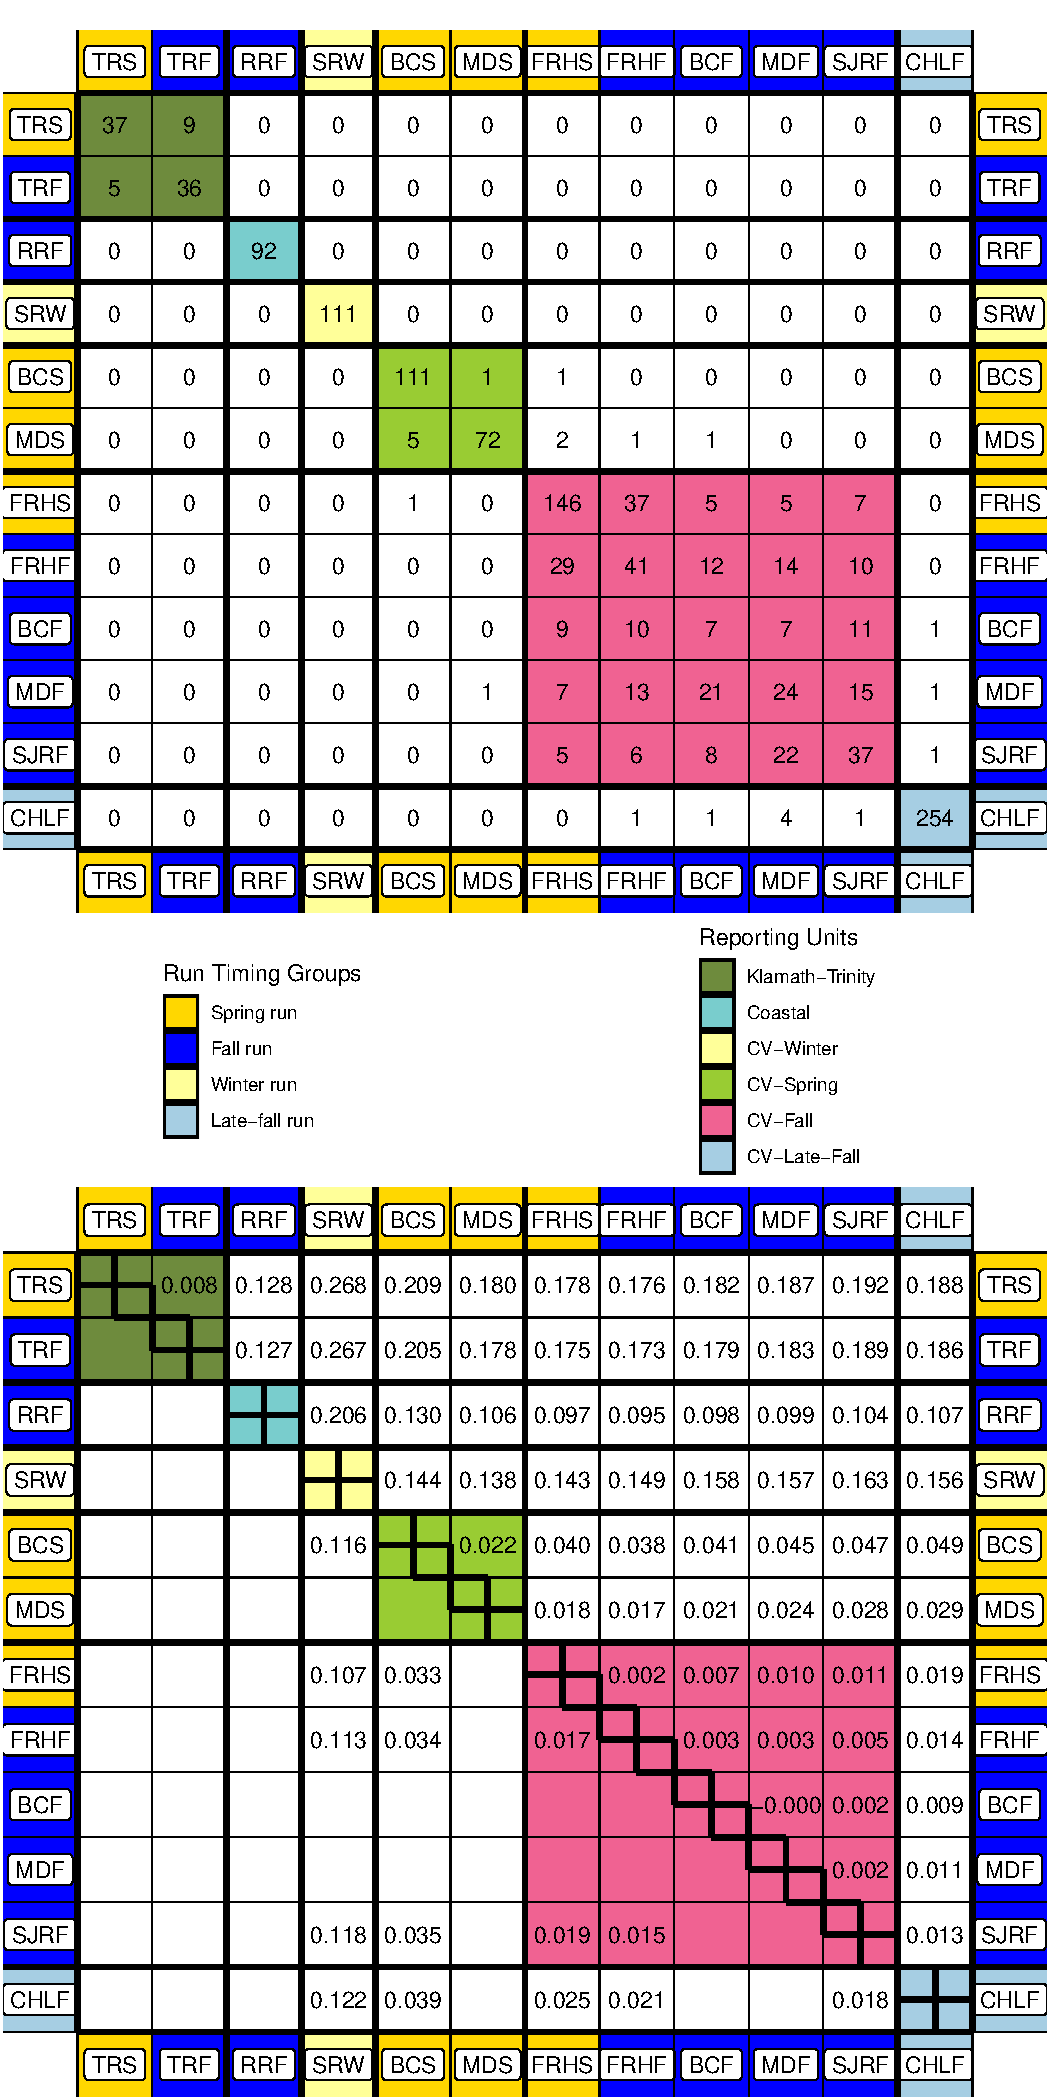
\includegraphics[width=\columnwidth]{images/gsi_and_fst_fig-crop.pdf}
\end{center}
\caption[\examplecap]{\examplecap}
\label{fig:example}
\end{figure}




\section*{Discussion}

When, and if, sequencing costs drop sufficiently, it may be possible to include
all different populations of a single species within a single standardized reference baseline
that performs equally well at broad and regional scales. A statistical approach for population
assignment from low coverage whole genome sequences appeared recently
\citep{desaixINPRESSpopulation}, and its authors noted that such a data type could
be ideal for producing reference baselines simultaneously applicable to broad scale
coverage and high resolution within sub-regions.   For the present, however,
baselines tailored to specific regions are essential for regional management questions.
It should be noted that recent 

